\clearpage
\cleardoublepage

\chapter{Skip Connections and Attention Mechanisms}

\section{Skip Connections}

Skip connections (shortcuts) bypass layers to enable gradient flow in deep networks.

\subsection{Residual Connections (ResNet)}

The residual learning framework:
\begin{equation}
\mathbf{y} = \mathcal{F}(\mathbf{x}) + \mathbf{x}
\end{equation}
where $\mathcal{F}$ is the learned residual mapping.

\begin{figure}[h]
    \centering
    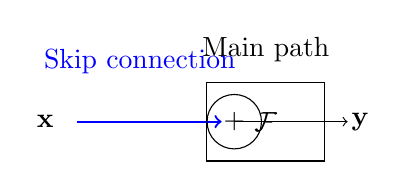
\begin{tikzpicture}[scale=0.8]
        % Main path
        \node[draw, rectangle, minimum width=1.5cm, minimum height=1cm] (F) at (2, 0) {$\mathcal{F}$};
        \node[above] at (2, 0.8) {Main path};
        
        % Skip connection
        \draw[->, thick, blue] (-1, 0) -- (1.3, 0);
        \node[above, blue] at (0, 0.6) {Skip connection};
        
        % Input/Output
        \node at (-1.5, 0) {$\mathbf{x}$};
        \node at (3.5, 0) {$\mathbf{y}$};
        
        % Addition
        \node[draw, circle] at (1.5, 0) {$+$};
        \draw[->] (1.5, 0) -- (3.3, 0);
    \end{tikzpicture}
    \caption{Residual connection}
    \label{fig:residual}
\end{figure}

If dimensions match: $\mathbf{y} = \mathcal{F}(\mathbf{x}, \{W_i\}) + \mathbf{x}$

If dimensions differ: $\mathbf{y} = \mathcal{F}(\mathbf{x}, \{W_i\}) + W_s\mathbf{x}$

\begin{properties}[ResNet Benefits]
\begin{itemize}
    \item Enables training of very deep networks (100+ layers)
    \item Alleviates vanishing/exploding gradients
    \item Reduces degradation problem
    \item Easy to implement and computationally minimal
\end{itemize}
\end{properties}

\subsection{Bottleneck Architecture}

Used in deeper ResNets to reduce complexity:
\begin{itemize}
    \item $1\times1$ conv to reduce dimensions
    \item $3\times3$ conv (bottleneck)
    \item $1\times1$ conv to restore dimensions
\end{itemize}

For input $C$, bottleneck outputs $C$:
\begin{enumerate}
    \item $\text{Conv }1\times1, C \rightarrow C//4$
    \item $\text{Conv }3\times3, C//4 \rightarrow C//4$
    \item $\text{Conv }1\times1, C//4 \rightarrow C$
\end{enumerate}

\subsection{Dense Connections (DenseNet)}

Each layer receives feature maps from all preceding layers:
\begin{equation}
\mathbf{x}_l = H_l([\mathbf{x}_0, \mathbf{x}_1, \ldots, \mathbf{x}_{l-1}])
\end{equation}

\begin{itemize}
    \item \textbf{Feature reuse:} Reduces parameters
    \item \textbf{Strong gradient flow}
    \item \textbf{Higher memory cost} due to concatenation
\end{itemize}

\section{Attention Mechanisms}

Attention allows models to focus on relevant parts of the input.

\subsection{Self-Attention}

The attention function:
\begin{equation}
\text{Attention}(\mathbf{Q}, \mathbf{K}, \mathbf{V}) = \text{softmax}\left(\frac{\mathbf{Q}\mathbf{K}^\top}{\sqrt{d_k}}\right)\mathbf{V}
\end{equation}

where:
\begin{itemize}
    \item $\mathbf{Q} = \mathbf{X}\mathbf{W}_Q$ (Query)
    \item $\mathbf{K} = \mathbf{X}\mathbf{W}_K$ (Key)
    \item $\mathbf{V} = \mathbf{X}\mathbf{W}_V$ (Value)
\end{itemize}

\begin{figure}[h]
    \centering
    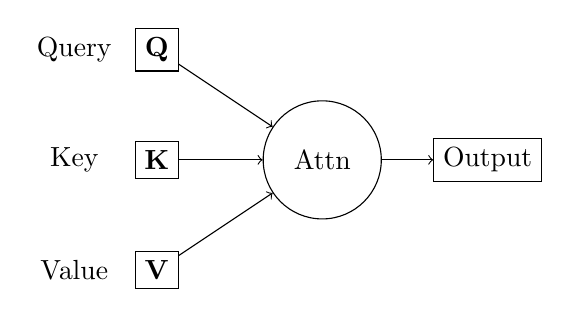
\begin{tikzpicture}[scale=0.7]
        % Q, K, V
        \node[draw, rectangle] (Q) at (-2, 2) {$\mathbf{Q}$};
        \node[draw, rectangle] (K) at (-2, 0) {$\mathbf{K}$};
        \node[draw, rectangle] (V) at (-2, -2) {$\mathbf{V}$};
        
        % Attention
        \node[draw, circle, minimum size=1.5cm] (attn) at (1, 0) {Attn};
        
        % Output
        \node[draw, rectangle] (out) at (4, 0) {Output};
        
        % Connections
        \draw[->] (Q) -- (attn);
        \draw[->] (K) -- (attn);
        \draw[->] (V) -- (attn);
        \draw[->] (attn) -- (out);
        
        % Labels
        \node at (-3.5, 2) {Query};
        \node at (-3.5, 0) {Key};
        \node at (-3.5, -2) {Value};
    \end{tikzpicture}
    \caption{Self-attention mechanism}
    \label{fig:self_attention}
\end{figure}

The scaling factor $\sqrt{d_k}$ prevents vanishing gradients for large $d_k$.

\begin{properties}[Self-Attention Properties]
\begin{itemize}
    \item \textbf{Allows modeling long-range dependencies}
    \item \textbf{Computationally $O(n^2)$ but parallelizable}
    \item \textbf{Interpretable:} Attention weights show relevance
\end{itemize}
\end{properties}

\subsection{Squeeze-and-Excitation (SE) Attention}

Channel attention mechanism:
\begin{enumerate}
    \item \textbf{Squeeze:} Global average pooling $\mathbf{z} = \frac{1}{H\times W}\sum_{i,j}\mathbf{X}_{:,i,j}$
    \item \textbf{Excitation:} FC-ReLU-FC-Sigmoid $\mathbf{s} = \sigma(W_2\delta(W_1\mathbf{z}))$
    \item \textbf{Scale:} $\tilde{\mathbf{X}} = \mathbf{s} \cdot \mathbf{X}$
\end{enumerate}

\begin{properties}[SE Block]
\begin{itemize}
    \item \textbf{Modeling channel dependencies}
    \item \textbf{Lightweight:} Minimal parameters
    \item \textbf{Plug-and-play:} Can be added to existing architectures
\end{itemize}
\end{properties}

\section{Chapter Summary}

\begin{enumerate}
    \item Skip connections enable deep networks by improving gradient flow
    \item Residual connections are the most widely used skip connection
    \item Attention mechanisms allow dynamic focus on relevant features
    \item Self-attention is the foundation of Transformers
    \item Channel attention (SE) provides efficient feature recalibration
\end{enumerate}
